\appendix



\begin{table}[h]
\centering
\captionsetup{justification=centering, margin = 1cm}
\begin{tabular}{l c c c c c c c c}
\hline
\textbf{Kategorie} & \multicolumn{3}{c}{\textbf{Community}} &  \multicolumn{3}{c}{\textbf{Distanz}} & \textbf{Anz. Trials} & \textbf{Vorh.}\\
& A & B & C & AB & BC & AC \\
\hline
1 & 1 & 1 & 1 & 1 & 1 & 3 & 18 & not B\\
2 & 1 & 1 & 1 & 1 & 2 & 3 & 12 & C\\
3 & 1 & 1 & 2 & 2 & 2 & 2 & 6 & C\\
4 & 1 & 1 & 2 & 1 & 2 & 1 & 12 & C\\
5 & 1 & 1 & 2 & 3 & 4 & 1 & 6 & not A\\
6 & 1 & 2 & 3 & 1 & 4 & 5 & 6 & C\\
7 & 1 & 2 & 3 & 4 & 4 & 4 & 18 & random\\
8 & 1 & 2 & 3 & 4 & 3 & 5 & 18 & A\\
\hline
\end{tabular}
\caption{Note. Anz. Trials = Anzahl der Durchgänge, Vorh. = Vorhersage, relevant für die Trefferquote}
\end{table}

\todo{BESCHREIBUNG DER TRIPLETS NOCH REIN?}

\paragraph{Stimulus-Set}
\captionsetup[subfigure]{labelformat=empty}
\begin{figure}
\begin{subfigure}{0.2\textwidth}
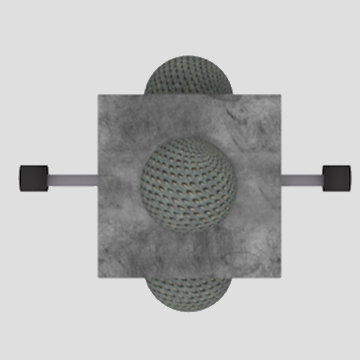
\includegraphics[width=\linewidth]{Bilder/Objekt1A.png}
\caption{Obj. 1, original} \label{fig:c}
\end{subfigure}\hspace{.5cm} %
\begin{subfigure}{0.2\textwidth}
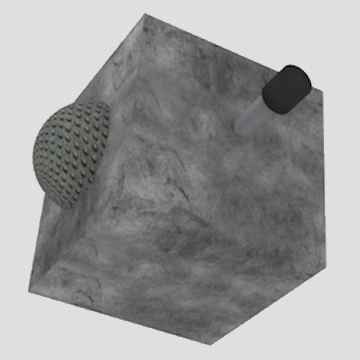
\includegraphics[width=\linewidth]{Bilder/Objekt1B.png}
\caption{Obj. 1, rotiert} \label{fig:d}
\end{subfigure} \hspace{.5cm}%
\begin{subfigure}{0.2\textwidth}
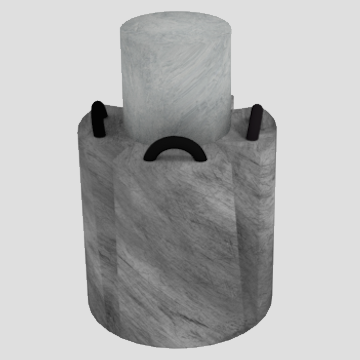
\includegraphics[width=\linewidth]{Bilder/Objekt2A.png}
\caption{Obj. 2, original} \label{fig:e}
\end{subfigure}\hspace{.5cm}
\begin{subfigure}{0.2\textwidth}
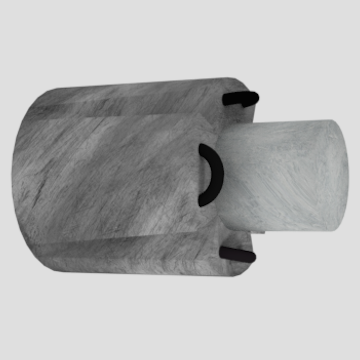
\includegraphics[width=\linewidth]{Bilder/Objekt2B.png}
\caption{Obj. 2, rotiert} \label{fig:f}
\end{subfigure}\hspace{.5cm}

\medskip
\begin{subfigure}{0.2\textwidth}
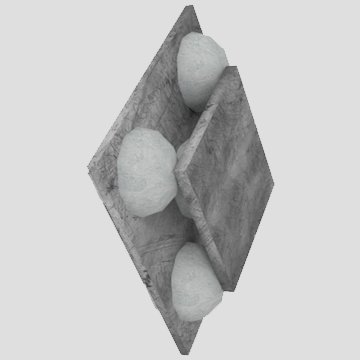
\includegraphics[width=\linewidth]{Bilder/Objekt3A.png}
\caption{Obj. 3, original} \label{fig:c}
\end{subfigure}\hspace{.5cm} %
\begin{subfigure}{0.2\textwidth}
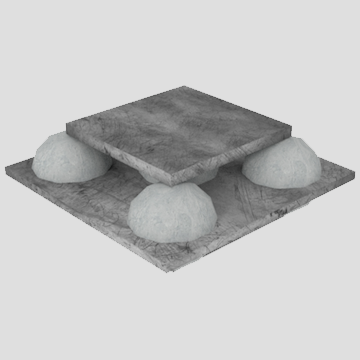
\includegraphics[width=\linewidth]{Bilder/Objekt3B.png}
\caption{Obj. 3, rotiert} \label{fig:d}
\end{subfigure} \hspace{.5cm}%
\begin{subfigure}{0.2\textwidth}
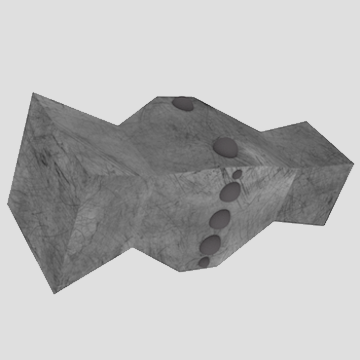
\includegraphics[width=\linewidth]{Bilder/Objekt4A.png}
\caption{Obj. 4, original} \label{fig:e}
\end{subfigure}\hspace{.5cm}
\begin{subfigure}{0.2\textwidth}
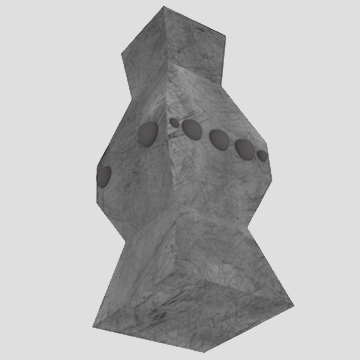
\includegraphics[width=\linewidth]{Bilder/Objekt4B.png}
\caption{Obj. 4, rotiert} \label{fig:f}
\end{subfigure}\hspace{.5cm}

\medskip
\begin{subfigure}{0.2\textwidth}
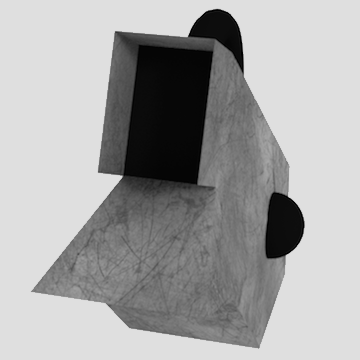
\includegraphics[width=\linewidth]{Bilder/Objekt5A.png}
\caption{Obj. 5, original} \label{fig:c}
\end{subfigure}\hspace{.5cm} %
\begin{subfigure}{0.2\textwidth}
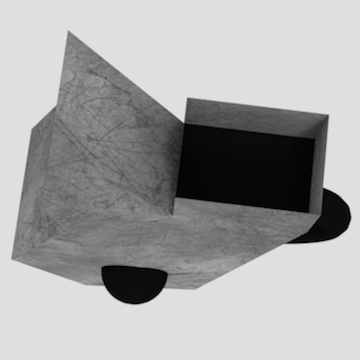
\includegraphics[width=\linewidth]{Bilder/Objekt5B.png}
\caption{Obj. 5, rotiert} \label{fig:d}
\end{subfigure} \hspace{.5cm}%
\begin{subfigure}{0.2\textwidth}
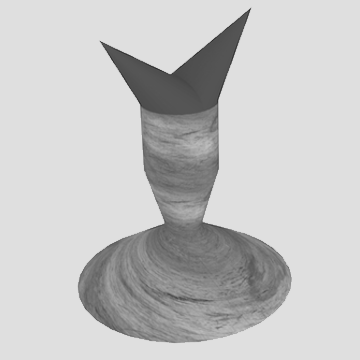
\includegraphics[width=\linewidth]{Bilder/Objekt6A.png}
\caption{Obj. 6, original} \label{fig:e}
\end{subfigure}\hspace{.5cm}
\begin{subfigure}{0.2\textwidth}
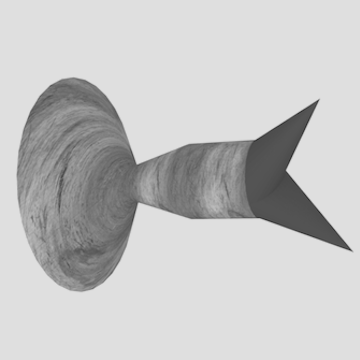
\includegraphics[width=\linewidth]{Bilder/Objekt6B.png}
\caption{Obj. 6, rotiert} \label{fig:f}
\end{subfigure}\hspace{.5cm}

\medskip
\begin{subfigure}{0.2\textwidth}
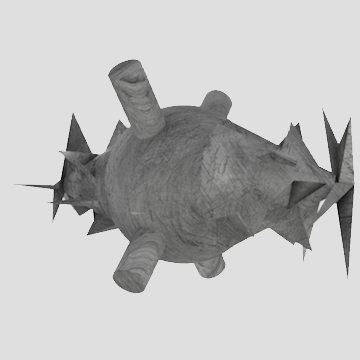
\includegraphics[width=\linewidth]{Bilder/Objekt7A.png}
\caption{Obj. 7, original} \label{fig:c}
\end{subfigure}\hspace{.5cm} %
\begin{subfigure}{0.2\textwidth}
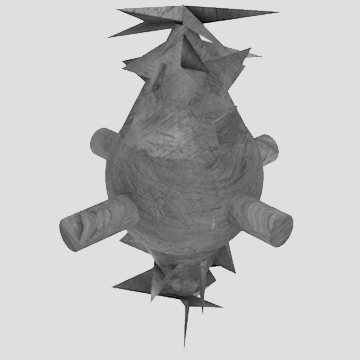
\includegraphics[width=\linewidth]{Bilder/Objekt7B.png}
\caption{Obj. 7, rotiert} \label{fig:d}
\end{subfigure} \hspace{.5cm}%
\begin{subfigure}{0.2\textwidth}
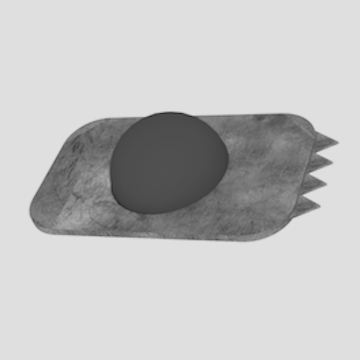
\includegraphics[width=\linewidth]{Bilder/Objekt8A.png}
\caption{Obj. 8, original} \label{fig:e}
\end{subfigure}\hspace{.5cm}
\begin{subfigure}{0.2\textwidth}
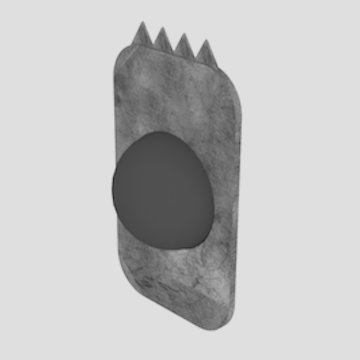
\includegraphics[width=\linewidth]{Bilder/Objekt8B.png}
\caption{Obj. 8, rotiert} \label{fig:f}
\end{subfigure}\hspace{.5cm}

\medskip
\begin{subfigure}{0.2\textwidth}
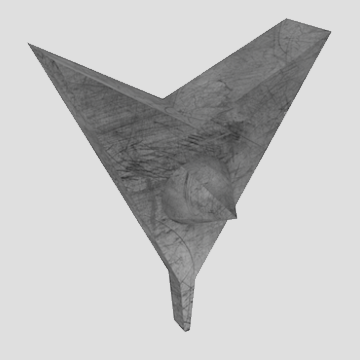
\includegraphics[width=\linewidth]{Bilder/Objekt9A.png}
\caption{Obj. 9, original} \label{fig:c}
\end{subfigure}\hspace{.5cm} %
\begin{subfigure}{0.2\textwidth}
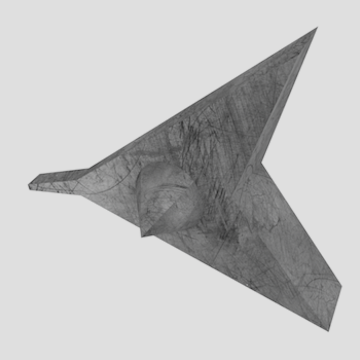
\includegraphics[width=\linewidth]{Bilder/Objekt9B.png}
\caption{Obj. 9, rotiert} \label{fig:d}
\end{subfigure} \hspace{.5cm}%
\begin{subfigure}{0.2\textwidth}
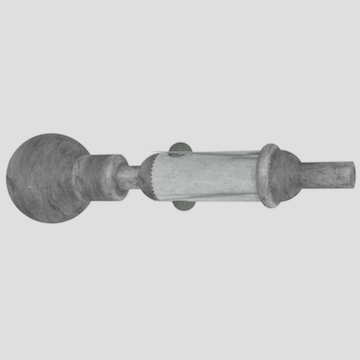
\includegraphics[width=\linewidth]{Bilder/Objekt10A.png}
\caption{Obj. 10, original} \label{fig:e}
\end{subfigure}\hspace{.5cm}
\begin{subfigure}{0.2\textwidth}
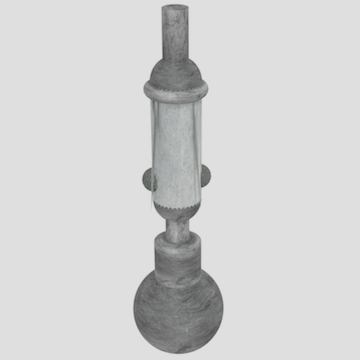
\includegraphics[width=\linewidth]{Bilder/Objekt10B.png}
\caption{Obj. 10, rotiert} \label{fig:f}
\end{subfigure}\hspace{.5cm}

\medskip
\begin{subfigure}{0.2\textwidth}
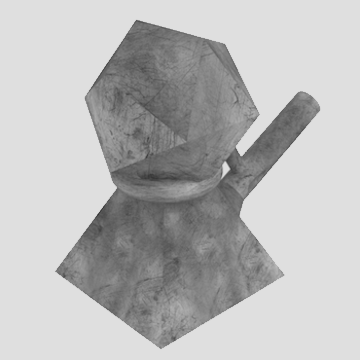
\includegraphics[width=\linewidth]{Bilder/Objekt11A.png}
\caption{Obj. 11, original} \label{fig:c}
\end{subfigure}\hspace{.5cm} %
\begin{subfigure}{0.2\textwidth}
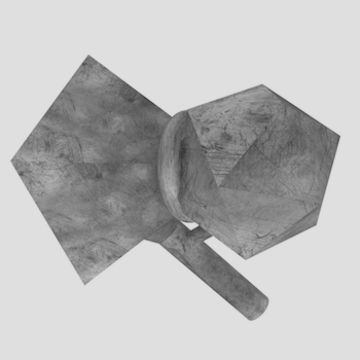
\includegraphics[width=\linewidth]{Bilder/Objekt11B.png}
\caption{Obj. 11, rotiert} \label{fig:d}
\end{subfigure} \hspace{.5cm}%
\begin{subfigure}{0.2\textwidth}
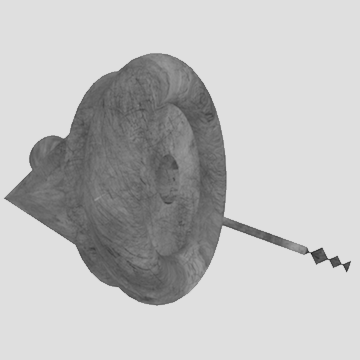
\includegraphics[width=\linewidth]{Bilder/Objekt12A.png}
\caption{Obj. 12, original} \label{fig:e}
\end{subfigure}\hspace{.5cm}
\begin{subfigure}{0.2\textwidth}
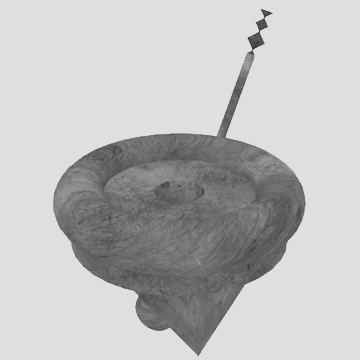
\includegraphics[width=\linewidth]{Bilder/Objekt12B.png}
\caption{Obj. 12, rotiert} \label{fig:f}
\end{subfigure}\hspace{.5cm}

\medskip
\begin{subfigure}{0.2\textwidth}
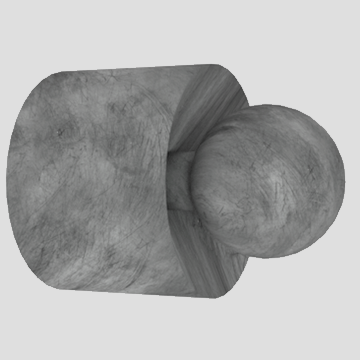
\includegraphics[width=\linewidth]{Bilder/Objekt13A.png}
\caption{Obj. 13, original} \label{fig:c}
\end{subfigure}\hspace{.5cm} %
\begin{subfigure}{0.2\textwidth}
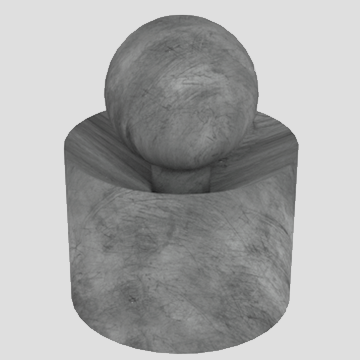
\includegraphics[width=\linewidth]{Bilder/Objekt13B.png}
\caption{Obj. 13, rotiert} \label{fig:d}
\end{subfigure} \hspace{.5cm}%
\begin{subfigure}{0.2\textwidth}
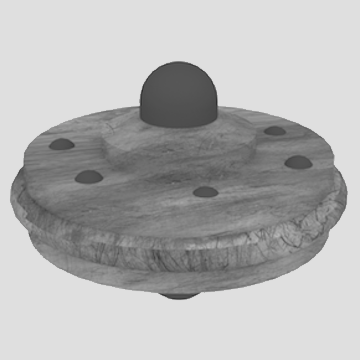
\includegraphics[width=\linewidth]{Bilder/Objekt14A.png}
\caption{Obj. 14, original} \label{fig:e}
\end{subfigure}\hspace{.5cm}
\begin{subfigure}{0.2\textwidth}
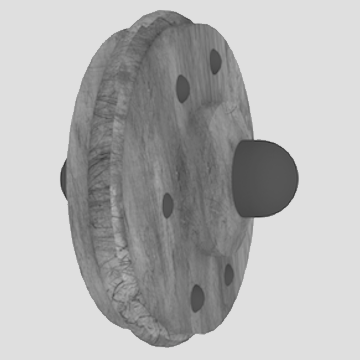
\includegraphics[width=\linewidth]{Bilder/Objekt14B.png}
\caption{Obj. 14, rotiert} \label{fig:f}
\end{subfigure}\hspace{.5cm}

\medskip
\begin{subfigure}{0.2\textwidth}
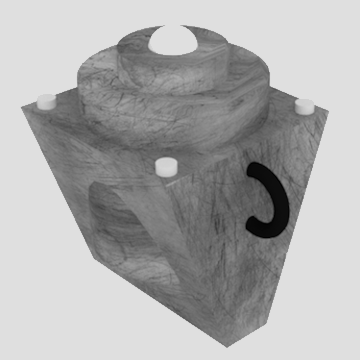
\includegraphics[width=\linewidth]{Bilder/Objekt15A.png}
\caption{Obj. 15, original} \label{fig:c}
\end{subfigure}\hspace{.5cm} %
\begin{subfigure}{0.2\textwidth}
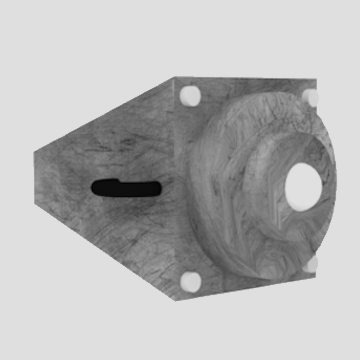
\includegraphics[width=\linewidth]{Bilder/Objekt15B.png}
\caption{Obj. 15, rotiert} \label{fig:d}
\end{subfigure} \hspace{.5cm}%
\begin{subfigure}{0.2\textwidth}
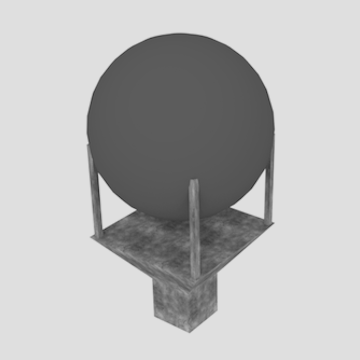
\includegraphics[width=\linewidth]{Bilder/Objekt16A.png}
\caption{Obj. 16, original} \label{fig:e}
\end{subfigure}\hspace{.5cm}
\begin{subfigure}{0.2\textwidth}
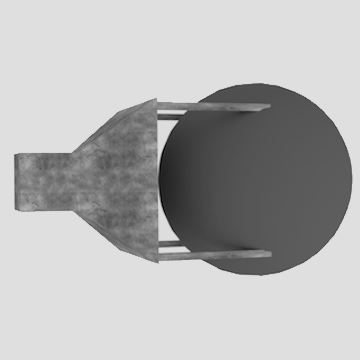
\includegraphics[width=\linewidth]{Bilder/Objekt16B.png}
\caption{Obj. 16, rotiert} \label{fig:f}
\end{subfigure}\hspace{.5cm}

\medskip
\begin{subfigure}{0.2\textwidth}
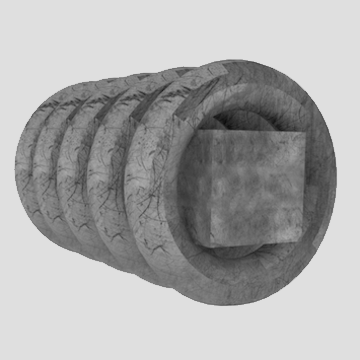
\includegraphics[width=\linewidth]{Bilder/Objekt17A.png}
\caption{Obj. 17, original} \label{fig:c}
\end{subfigure}\hspace{.5cm} %
\begin{subfigure}{0.2\textwidth}
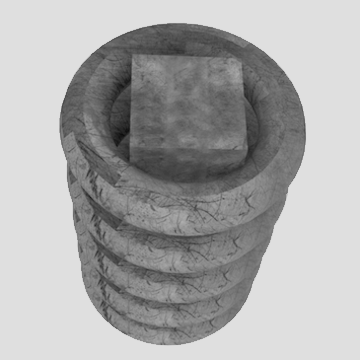
\includegraphics[width=\linewidth]{Bilder/Objekt17B.png}
\caption{Obj. 17, rotiert} \label{fig:d}
\end{subfigure} \hspace{.5cm}%
\begin{subfigure}{0.2\textwidth}
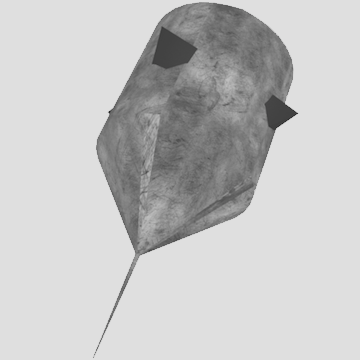
\includegraphics[width=\linewidth]{Bilder/Objekt18A.png}
\caption{Obj. 18, original} \label{fig:e}
\end{subfigure}\hspace{.5cm}
\begin{subfigure}{0.2\textwidth}
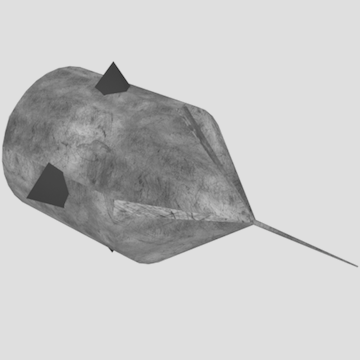
\includegraphics[width=\linewidth]{Bilder/Objekt18B.png}
\caption{Obj. 18, rotiert} \label{fig:f}
\end{subfigure}\hspace{.5cm}

\caption{My complicated figure} \label{fig:1}
\end{figure}

